%!TEX root = comps_NKasimov.tex
\chapter{High Fidelity Simulation Results}
\label{chapter:4}
In this chapter one can find  the results of benchmarking for CBVP applied to simple testing problem --- Heat equation with different boundary conditions at the wall (Dirichlet, Neumann, Robin), as well as results of Hi-Fi simulations with the use of CBVP for flows around different number and types of obstacles.

\section{Benchmark of using Characteristic Based Volume Penalization}
Applicability of CBVP on different BC was tested on 1D heat equation \eqref{eq:heat}. 
\begin{align}
\frac {\pt T}{\pt t} &= k \frac {\pt^2 T}{\pt x^2}. \label{eq:heat}
\end{align}
On the right domain boundary the wall was placed, so one can observe reflection of the incident wave using CBVP and compare it to exact solution. The main error controlling parameter in CBVP is penalization parameter $\eta$, so it was varied to achieve convergence with exact solution.

\subsection{Dirichlet Boundary Condition}
This boundary condition \eqref{eq:heat_dirichlet}, also called isothermal boundary condition, specifies temperature (integrated variable for heat equation) as a constant value at the obstacle/wall interface. In this particular benchmark the value was equal to 0.
\begin{align}
\vbr T_{wall} = 0 \qquad \implies \qquad \frac {\pt T}{\pt t} &= k \frac {\pt^2 T}{\pt x^2} - \frac \chi \eta_b T. \label{eq:heat_dirichlet}
\end{align}
Varying penalization parameter $\eta_b$ led to solutions with different accuracy (see Fig.~\ref{fig:heat_dirichlet}).
\begin{figure}[h!]
\centering 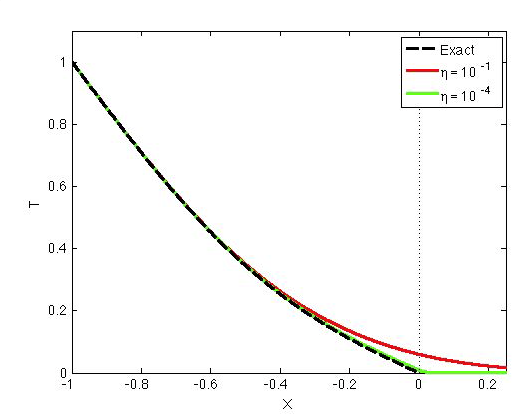
\includegraphics[scale=0.6]{fig/heat_dirichlet.png}\\
\caption{Temperature profile at the end of simulation. Dirichlet boundary condition. \label{fig:heat_dirichlet}}
\end{figure}\\
One can see that $\eta_b = 10^{-4}$ converges to the exact solution well. In fact, rate of convergence for this simulation is $\sqrt{\eta_b}$ \cite{ebd_nk_ovv_cbvp_jcp}, since it is Brinkman type penalization \cite{lib:vp_liu}.

\subsection{Neumann Boundary Condition}
This boundary condition \eqref{eq:heat_neumann} specifies constant rate of heat amount going in to or out of the system. In case of zero rate it is called adiabatic boundary condition. In this benchmark latter was considered.
\begin{align}
\vbr{\frac {\pt T}{\pt x}}_{wall} = 0 \qquad \implies \qquad \frac {\pt T}{\pt t} &= (1-\chi)k \frac {\pt^2 T}{\pt x^2} - \frac \chi \eta_c \frac {\pt T}{\pt x}. \label{eq:heat_neumann}
\end{align}
Analogously to Dirichlet BC, varying penalization parameter $\eta_c$ led to different accuracy of the solution (see Fig.~\ref{fig:heat_neumann}). Rate of convergence for this type of simulations is $\eta_c$ \cite{ebd_nk_ovv_cbvp_jcp}. One can notice that penalization parameter for Neumann type BC is different than for Dirichlet type BC, which is connected to different time scales of the processes. In case of BP solution at the boundary decays inside of the obstacle, on the other hand for characteristic BC solution is translated inside of the obstacle. 
\begin{figure}[h!]
\centering 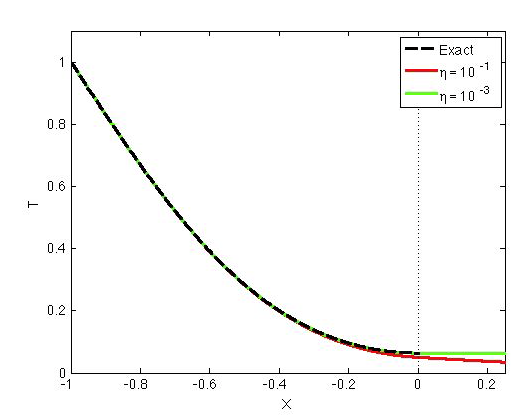
\includegraphics[scale=0.6]{fig/heat_neumann.png}\\
\caption{Temperature profile at the end of simulation. Neumann boundary condition. \label{fig:heat_neumann}}
\end{figure}

\subsection{Robin Boundary Condition}
Last benchmark problem was to mimic Robin boundary condition at the obstacle interface, when both the solution value and its derivative are specified at the boundary. In this particular problem \eqref{eq:heat_robin} was used as a BC.
\begin{align}
T + 2 \frac {\pt T}{\pt x} = 5 \qquad \implies \qquad \frac {\pt T}{\pt t} &= (1-\chi)k \frac {\pt^2 T}{\pt x^2} - \frac \chi {\eta_r} \rbr{T + 2 \frac {\pt T}{\pt x} - 5}. \label{eq:heat_robin}
\end{align}
In this type of simulations rate of convergence was predominated due to characteristic based terms as $\eta_r$ \cite{ebd_nk_ovv_cbvp_jcp} (see Fig.~\ref{fig:heat_robin}).
\begin{figure}[h!]
\centering 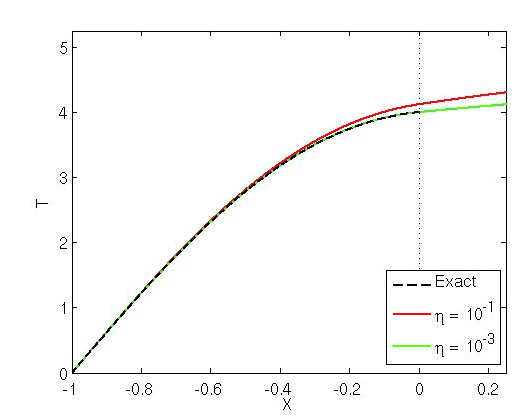
\includegraphics[scale=0.6]{fig/heat_robin.png}\\
\caption{Temperature profile at the end of simulation. Robin boundary condition. \label{fig:heat_robin}}
\end{figure} 

\section{Simulation Results}
After the method was validated and convergence rates were studied, variety of 2D simulations of supersonic inviscid flow were performed. Namely, flow around single and multiple stationary and moving cylinders, wedges with subcritical and supercritical angles. It is worth to mention that at this point no quantitative analysis of applicability of CBVP was done for these simulations. All results are treated based on the assumption that convergence rates defined in heat equation benchmarks hold for these simulations according to the used BCs (either $\sim \sqrt \eta$ or $\sim \eta$). 

{\color{red}{All of our results here, for cylinders, wedge, etc, split by subsections}}






